\section{\EdgeQuantum Design}
\label{sec:design}

%In this section, we present the design of \EdgeQuantum, a tiered-memory quantum circuit simulator specifically optimized for resource-constrained edge devices. 
%\EdgeQuantum overcomes the physical memory limitations of edge hardware not by simplifying the quantum circuit, but by implementing a hierarchical memory management system that treats NVMe SSD as a direct extension of the GPU memory.
%By utilizing Unified Virtual Memory (UVM) as a zero-copy staging buffer and implementing a 4-buffer asynchronous pipeline, \EdgeQuantum enables the simulation of state vectors up to 4\,TB (39 qubits) on devices with only 8\,GB of RAM.


\begin{figure}[t]
    \centering
    % Ensure you have this file or use a placeholder
    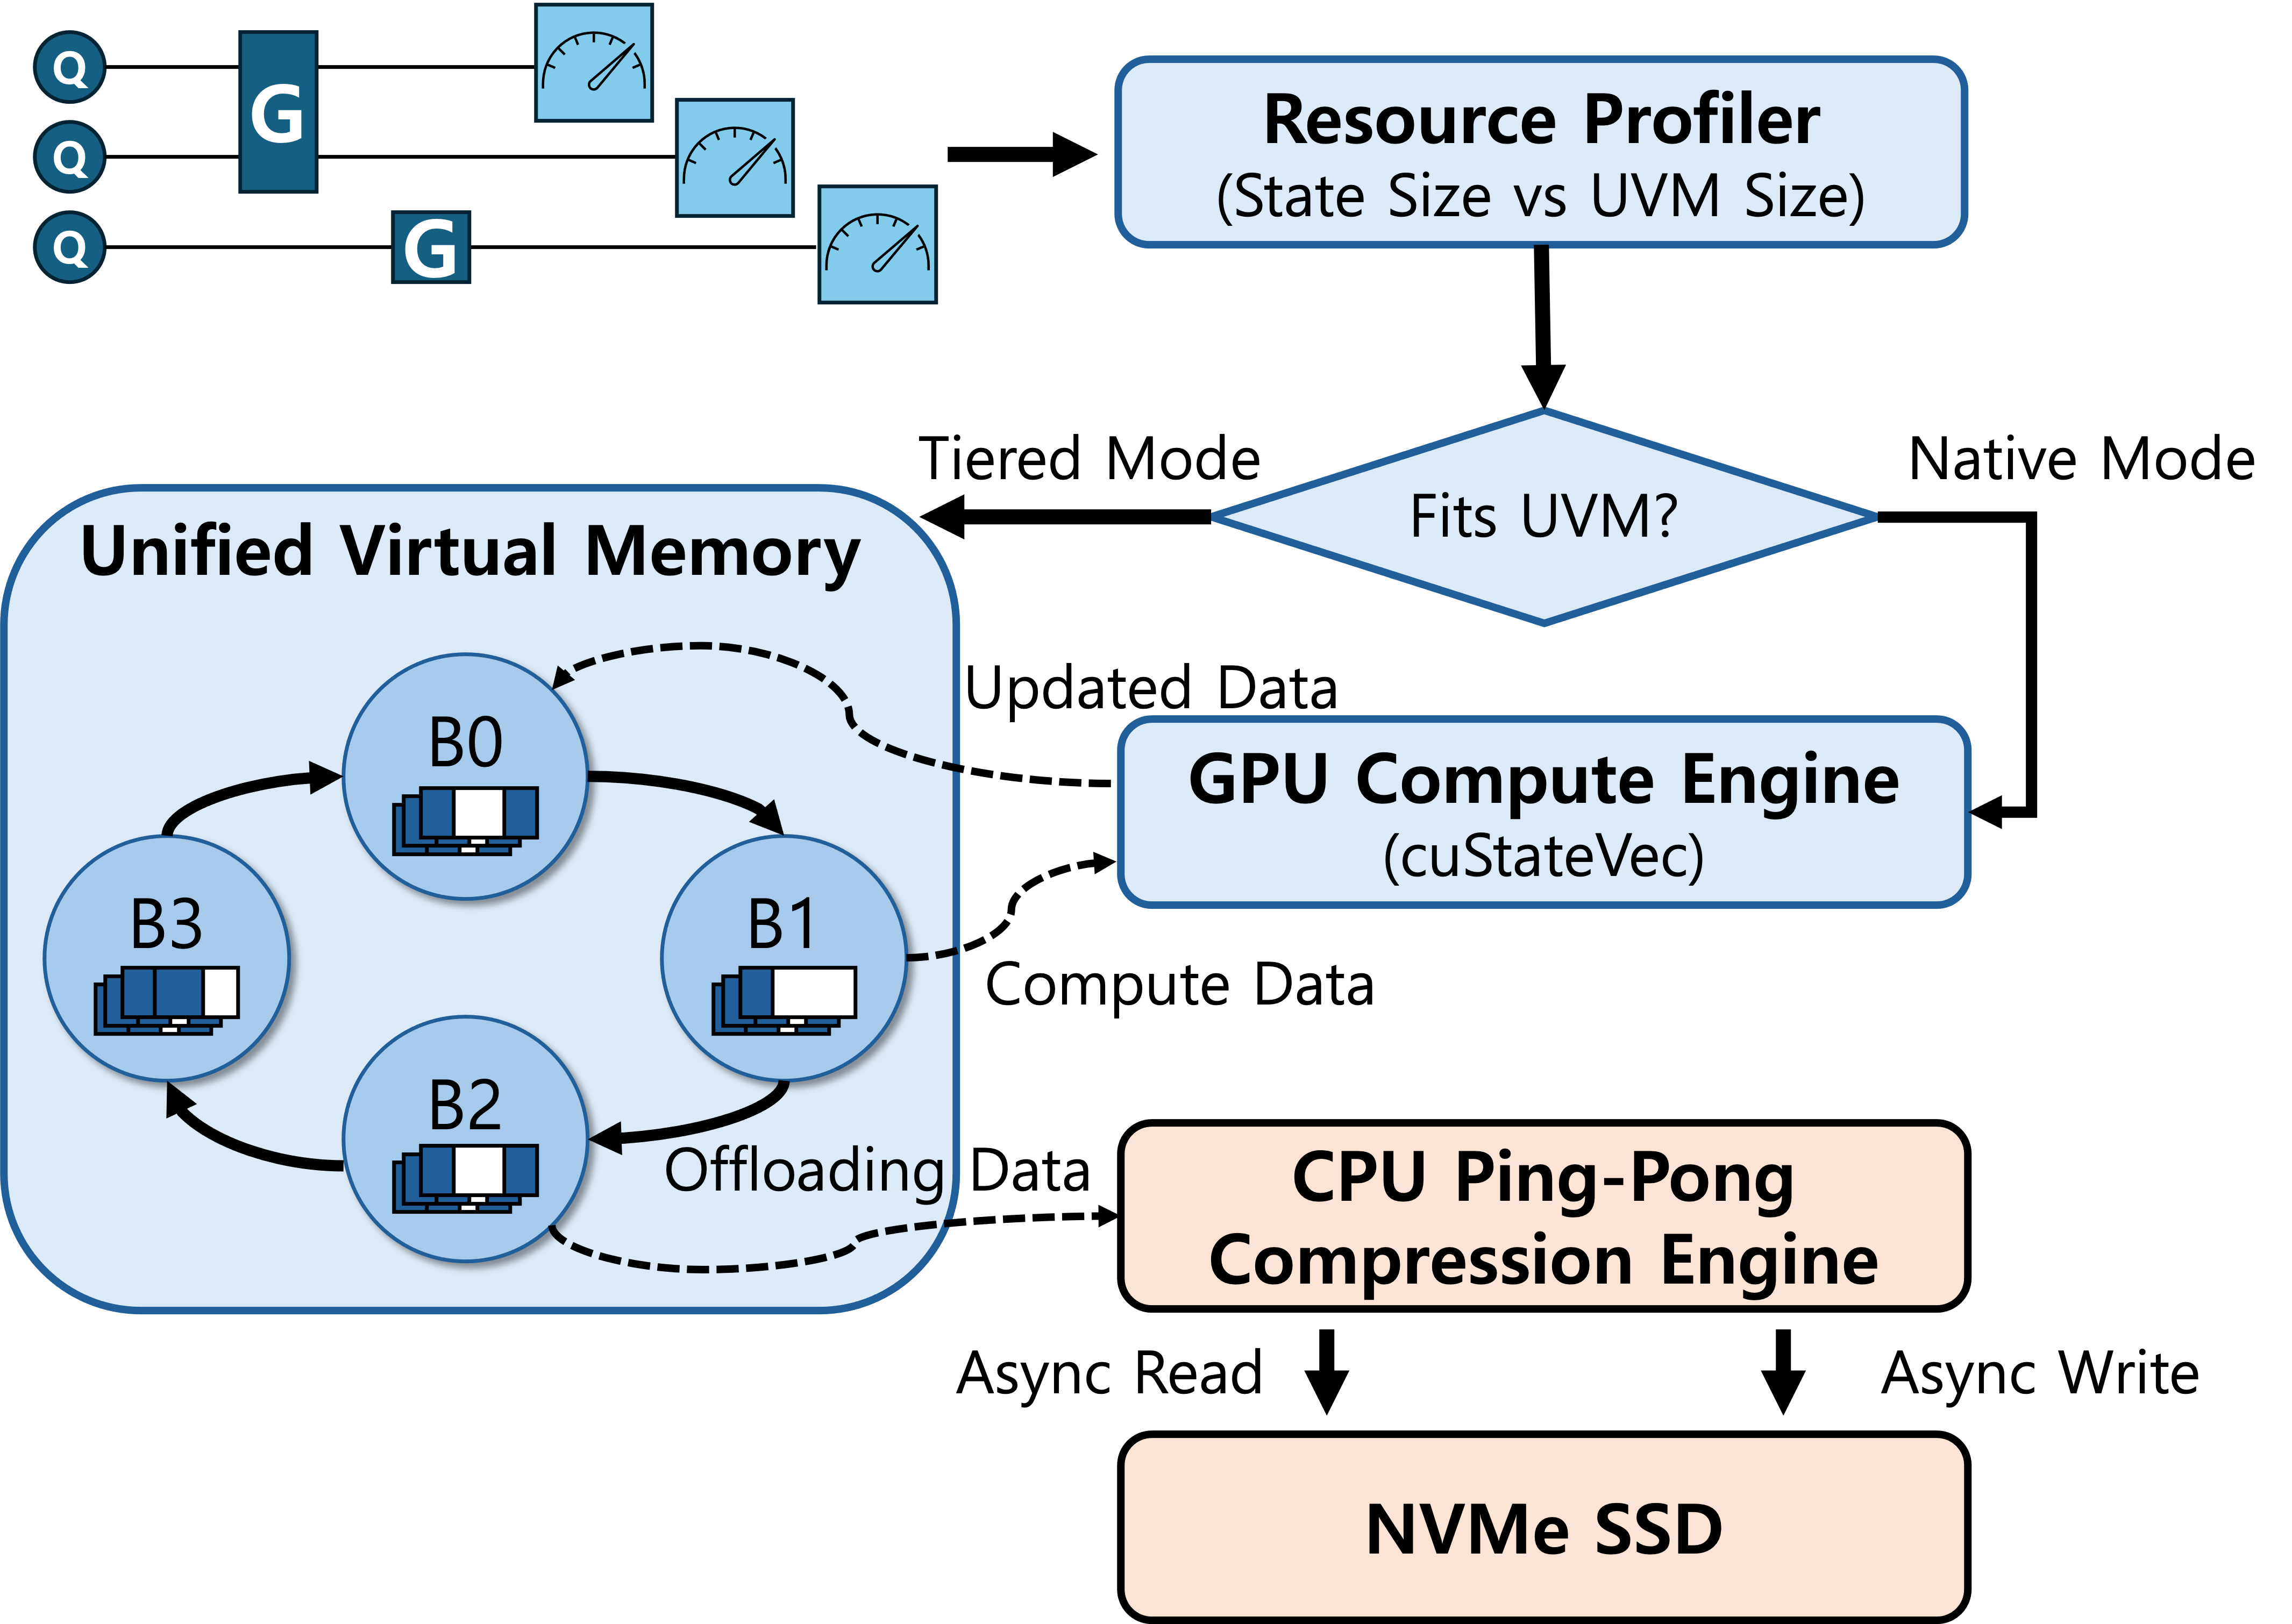
\includegraphics[width=0.85\columnwidth]{Figures/architecture_edge.png}
    \caption{Overall architecture of \EdgeQuantum.}
        \vspace{-.2cm}
    \label{overall_architecture}
\end{figure}



\subsection{Overall Procedure}
\label{design_overall}

Figure~\ref{overall_architecture} shows the overall procedure of \EdgeQuantum.
\EdgeQuantum processes a quantum circuit simulation through dynamic resource profiling and a Unified Virtual Memory (UVM)-based storage pipeline.

\noindent\textbf{Resource Profiling and Mode Selection.}
When a quantum circuit simulation starts, \textit{Resource Profiler} computes the state vector size and compares it with available memory. To prevent mid-execution out-of-memory (OOM) crashes, this comparison uses 80\% of available GPU memory as a threshold, reserving headroom for kernel workspaces and runtime allocations. Based on this comparison, \EdgeQuantum determines whether the state vector fits within available memory. If the state vector fits within available memory, \EdgeQuantum operates in \textit{Native Mode}. In this mode, \textit{GPU Compute Engine} allocates the state in memory and executes the simulation using \textit{cuStateVec}. If the state vector exceeds available memory, \EdgeQuantum activates \textit{Tiered Mode}, which uses NVMe SSD as a memory hierarchy extension. By selecting the execution path based on capacity, \EdgeQuantum utilizes available hardware and prevents OOM failures.

\noindent\textbf{Tiered Mode Execution.}
In \textit{Tiered Mode}, \EdgeQuantum employs a 4-buffer UVM pipeline that establishes a zero-copy data path through the Unified Memory Architecture (UMA), avoiding host-to-device overheads of existing simulators. The state vector is partitioned into fixed-size chunks staged through four UVM ring buffers (B0-B3). During execution, \textit{GPU Compute Engine} applies gates on UVM ring buffers, while \textit{CPU Ping-Pong Compression Engine} performs async I/O between NVMe SSD and buffers. The 4-buffer depth absorbs NVMe's asymmetric read/write latency by overlapping GPU compute on one buffer with CPU I/O on others, preventing pipeline stalls. The compression engine engages dual-file ping-pong compression when the state vector exceeds SSD capacity ($\geq$36 qubits), enabling \EdgeQuantum to simulate quantum systems (e.g., 39 qubits) that exceed physical storage capacity.



\subsection{Tiered Memory Architecture with UVM}
\label{design_memory}



A fundamental challenge in edge out-of-core simulation is the redundant host-to-device copies imposed by standard CUDA frameworks. On NVIDIA Jetson platforms, the CPU and GPU share a DRAM pool under UMA, enabling zero-copy data paths. Figure~\ref{uvm_diff} shows how \EdgeQuantum leverages UMA via UVM visibility control to establish an efficient data path.

\noindent\textbf{Existing Storage-backed Execution. }Despite the shared DRAM on UMA platforms, existing quantum simulation frameworks rely on standard device memory allocation models. As shown at the top of Figure~\ref{uvm_diff}, using standard device memory allocation (e.g., \texttt{cudaMalloc}) enforces a logical separation between host and device memory spaces. When retrieving state vector chunks from storage, POSIX I/O system calls (e.g., \texttt{pread}) cannot perform Direct Memory Access (DMA) into device memory. The system stages the data in an intermediate host-side buffer, followed by an explicit \texttt{cudaMemcpy} (H2D). This data path has two limitations for resource-constrained edge devices. First, it doubles the physical memory footprint (2$\times$ Memory constraint). Second, the additional memory copy operation saturates memory bandwidth and reduces simulation throughput.


\begin{figure}[t]
    \centering
    % Ensure you have this file or use a placeholder
    \includegraphics[width=0.85\columnwidth]{Figures/test_uvm.png}
    \caption{Data path comparison. (Top) Existing execution. (Bottom) \EdgeQuantum's zero-copy execution on UMA.}
    \vspace{-.2cm}
    \label{uvm_diff}
\end{figure}

\noindent\textbf{Zero-copy Execution for UMA. }To remove this bottleneck, \EdgeQuantum designs a zero-copy data path by controlling the visibility of UVM at the OS and driver level. As shown at the bottom of Figure~\ref{uvm_diff}, \EdgeQuantum allocates simulation buffers using \texttt{cudaMallocManaged} with the \texttt{cudaMemAttachHost} flag. This flag maps physical pages into the CPU page tables. With CPU-side visibility, \EdgeQuantum performs \texttt{O\_DIRECT} file operations, streaming state vector chunks directly into the UVM ring buffer while bypassing the Linux page cache and avoiding memory pollution. Before quantum gate execution, \EdgeQuantum issues a \texttt{cudaStreamAttachMemAsync} with \texttt{cudaMemAttachGlobal} flag. This asynchronous operation updates the GPU Memory Management Unit (MMU) page tables without data migration and transfers ownership of the physical DRAM pages to \textit{GPU Compute Engine}. By managing these UVM visibility transitions within a ring-buffer structure, \EdgeQuantum ensures that active data residency remains within physical DRAM limits, thereby preventing OS-level thrashing and removing explicit memory copies.



\subsection{4-Buffer Asynchronous Pipeline}
\label{design_pipeline}



%The primary performance bottleneck in out-of-core quantum simulation on edge devices is the asymmetric I/O latency of commodity NVMe SSDs. While sequential reads sustain 1.38~GB/s, writes are limited to 1.0~GB/s (Section~\ref{back2}). Traditional out-of-core simulators issue concurrent asynchronous reads and writes without considering this asymmetry. This bidirectional I/O causes NVMe controller contention and degrades throughput. To mitigate this hardware limitation, \EdgeQuantum implements an asynchronous pipeline governed by an \textit{I/O Serialization Policy}. 

The primary bottleneck in out-of-core quantum simulation on edge devices is the asymmetric I/O latency of NVMe SSDs (Section~\ref{back2}). Existing simulators issue concurrent reads and writes, ignoring this asymmetry. This bidirectional I/O causes controller contention and degrades throughput. To mitigate this, \EdgeQuantum implements an asynchronous pipeline with an \textit{I/O Serialization Policy}. 

\noindent\textbf{Pipeline Architecture.} Figure~\ref{design_3.3} shows the execution timeline of the asynchronous pipeline. The core design principle is to isolate I/O directions to preserve NVMe bandwidth while overlapping them with independent GPU computation. This isolation is enforced by an I/O serialization barrier, ensuring a new read is blocked until the preceding write completes. This 4-buffer configuration is selected based on the latency relationship between NVMe writes ($T_{write} \approx 256$ms for a 256 MB chunk at the measured 1.0 GB/s) and the combined read-compute window ($T_{read} + T_{compute}$). We adopt a 4-buffer depth to provide headroom against write-latency variability, ensuring a free UVM ring buffer is available for the next $T_{read}$ phase. Driven by this policy, \EdgeQuantum processes state vector chunk $k$ through the following sequence:

\begin{figure}[t]
    \centering
    % Ensure you have this file or use a placeholder
    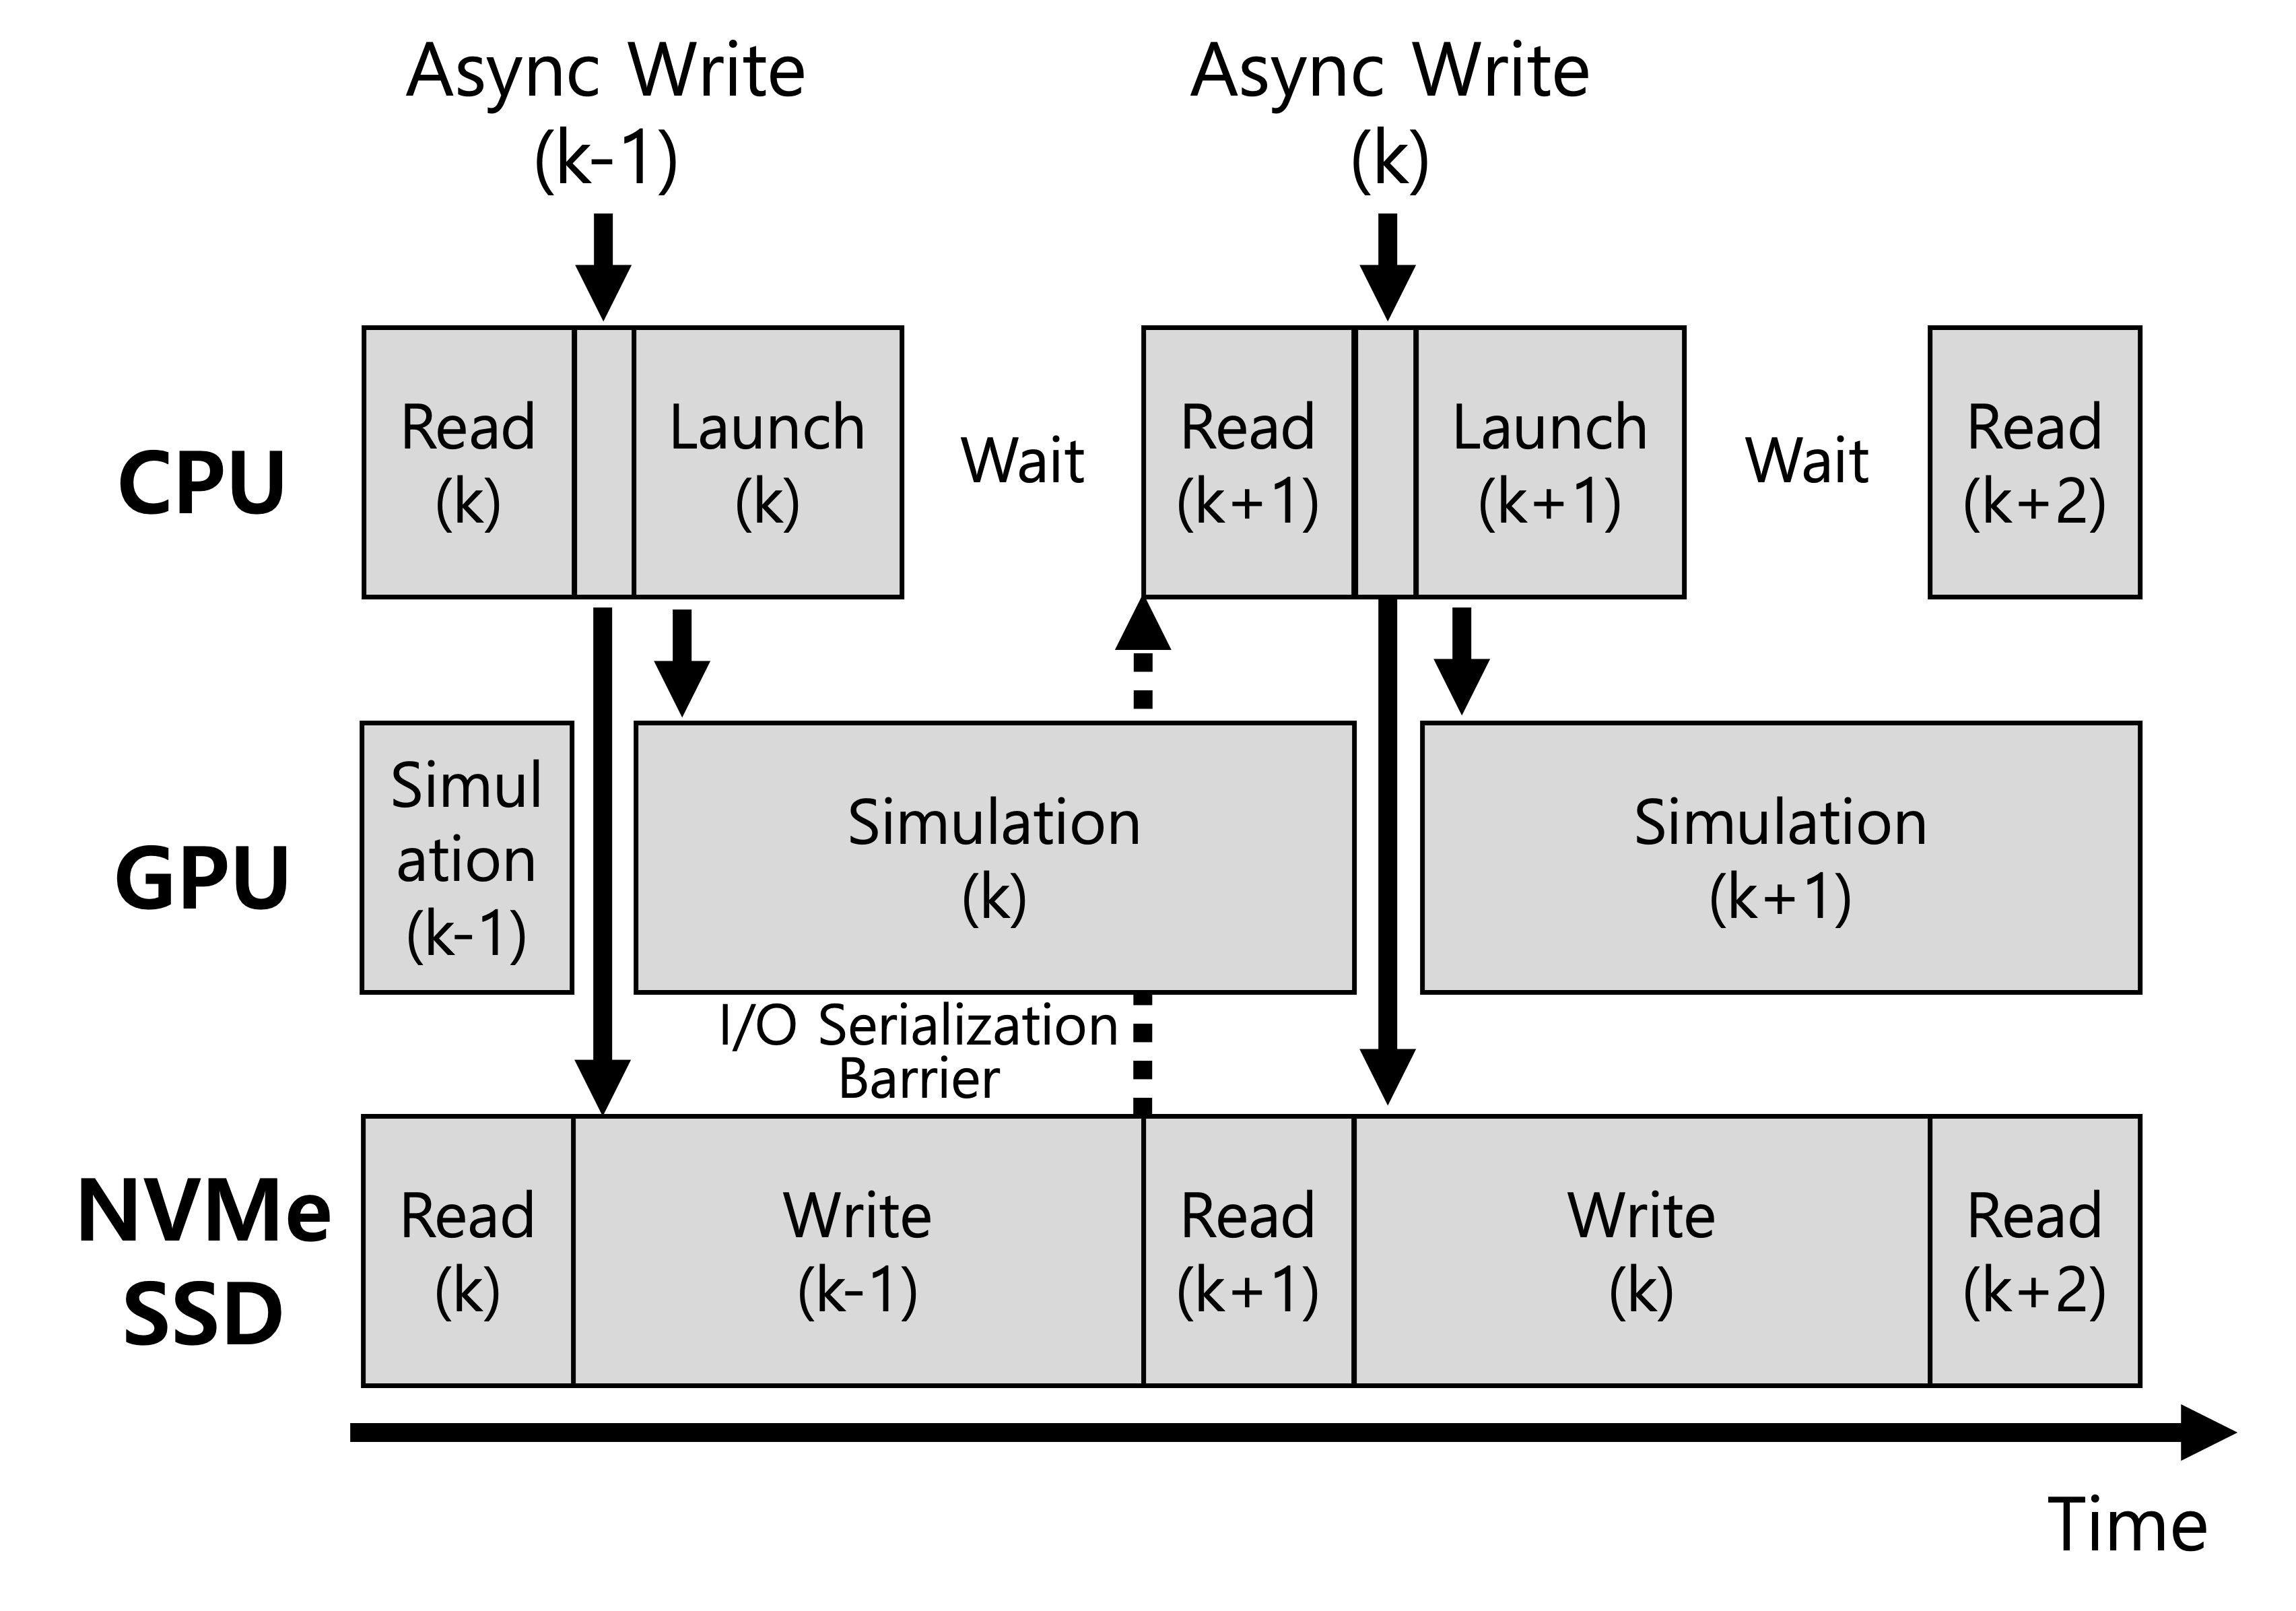
\includegraphics[width=0.85\columnwidth]{Figures/edge_design3.3.png}
    \caption{Execution timeline of the asynchronous pipeline. The dotted line marks the I/O serialization barrier.}
    \vspace{-.2cm}
    \label{design_3.3}
\end{figure}


\begin{enumerate}
\item \textbf{I/O Serialization Barrier:} To avoid bidirectional I/O contention, the CPU halts at a barrier until the background \texttt{pwrite} of an earlier chunk (e.g., $k-2$) completes. This stalling prevents the OS block layer from mixing read/write queues and avoids triggering NVMe garbage collection that delays the subsequent read.
\item \textbf{Synchronous Read:} After clearing the barrier, \EdgeQuantum issues a synchronous \texttt{pread} to load chunk $k$ directly into the UVM ring buffer at sequential read bandwidth.
\item \textbf{Asynchronous Write:} After the read, the framework dispatches a background thread to asynchronously write the previously computed chunk ($k-1$) back to storage.
\item \textbf{GPU Compute Overlap:} Concurrently with the background write, \textit{GPU Compute Engine} executes gate kernels on chunk $k$. Because the Jetson SoC has independent memory and NVMe controllers, computation overlaps with the storage write. This hardware-level separation ensures CPU-intensive I/O and GPU-intensive kernels operate without interference.
\end{enumerate}
By serializing the I/O path and overlapping GPU execution, \EdgeQuantum hides write latency without causing bandwidth contention. 

\noindent\textbf{Cross-Chunk Gate Handling.} Local gates act on amplitudes within a single chunk and are processed within one UVM ring buffer ($q < \log_2(\text{chunk size})$). In contrast, gates targeting qubits beyond the chunk boundary couple amplitudes residing in different chunks, which must be co-resident in memory before invocation. For gates spanning the chunk boundary ($q \geq \log_2(\text{chunk size})$), \EdgeQuantum streams the chunk pair $(c, c \oplus 2^{q-\log_2(\text{chunk size})})$ into two adjacent UVM ring buffers and invokes \textit{cuStateVec} on the paired amplitudes. This pair-wise handling extends to two-global-qubit gates by occupying four ring buffers, matching the 4-buffer depth. Although cross-chunk gates double the per-gate I/O, the asynchronous pipeline overlaps the additional read with GPU compute on the prior pair, preserving throughput characteristics of the local-gate case. Thus, the 4-buffer choice supports both the asynchronous pipeline and cross-chunk gate handling without requiring additional buffers.





\subsection{LZ4 Ping-Pong Compression}
\label{design_compression}
\begin{algorithm}[t]
\caption{Dynamic Ping-Pong Compression Strategy}
\scriptsize
\label{alg:pingpong}
\begin{algorithmic}[1]
\Require Gate Layer $L$, Total Chunks $M$, Truncation Depth $T$
\Ensure Compressed state vector is updated for Layer $L+1$

\State $OffsetOut \gets 0$
\If{$L \bmod 2 = 0$} \Comment{Swap files each layer}
    \State $FileIn, FileOut \gets$ FileA, FileB
    \State $IdxIn, IdxOut \gets$ IndexA, IndexB
\Else
    \State $FileIn, FileOut \gets$ FileB, FileA
    \State $IdxIn, IdxOut \gets$ IndexB, IndexA
\EndIf

\For{$c = 0$ \textbf{to} $M-1$}
    \State $OffsetIn \gets IdxIn[c]$ \Comment{Variable-size read}
    \State $SizeIn \gets IdxIn[c+1] - OffsetIn$
    \State $CompBuf \gets$ \textsc{AsyncRead}$(FileIn, OffsetIn, SizeIn)$
    \State $ShufBuf \gets$ \textsc{LZ4Decompress}$(CompBuf)$ \Comment{Decompress shuffled chunk}
    \State $UVMBuf \gets$ \textsc{ByteUnshuffle}$(ShufBuf)$ \Comment{Restore interleaved float32}
    \State \textsc{GPUCompute}$(UVMBuf)$ \Comment{Apply gates (cross-chunk uses chunk pair)}
    \State \textsc{MantissaTruncate}$(UVMBuf, T)$ \Comment{Zero lower $(23-T)$ mantissa bits}
    \State $ShufBuf \gets$ \textsc{ByteShuffle}$(UVMBuf)$ \Comment{Group same-position bytes}
    \State $SizeOut \gets$ \textsc{LZ4Compress}$(ShufBuf, CompBuf)$ 
    \State \textsc{AsyncWrite}$(FileOut, CompBuf, OffsetOut, SizeOut)$ 
    \State $IdxOut[c] \gets OffsetOut$ \Comment{Update index}
    \State $OffsetOut \gets OffsetOut + SizeOut$
\EndFor
\State $IdxOut[M] \gets OffsetOut$ \Comment{Record total size}

\end{algorithmic}
\end{algorithm}
 

For quantum simulations where the logical state vector exceeds NVMe capacity (e.g., $N \ge 36$ qubits requires $\ge 512$~GB), raw storage becomes a bottleneck. To extend simulation beyond storage limits, \EdgeQuantum integrates a three-stage compression layer combining mantissa truncation, byte shuffle, and LZ4 for low-overhead structure-aware float32 compression. This layer reduces I/O volume by trading CPU cycles for compression overhead. However, gate operations modify the state vector, changing chunk entropy and producing unpredictable compressed sizes. This makes in-place updates infeasible and causes entropy-driven fragmentation.

To address this fragmentation, we design a dynamic ping-pong strategy detailed in Algorithm~\ref{alg:pingpong}. The strategy swaps two backing files, \textit{File A} and \textit{File B}, at the start of each gate layer \textbf{(Lines 2-7)} to enforce atomic updates. During the simulation loop \textbf{(Lines 8-20)}, the framework executes a compressed pipeline for each chunk $c$. First, \EdgeQuantum retrieves the variable-sized compressed chunk via $IdxIn$, decompresses, and reverts the byte shuffle to restore the float32 layout in the UVM ring buffer \textbf{(Lines 9-13)}. Next, \textit{GPU Compute Engine} applies gates to the UVM ring buffer, overlapping with I/O of adjacent chunks \textbf{(Line 14)}. Then, the framework truncates the lower $(23-T)$ mantissa bits, applies byte shuffle to same-position bytes across amplitudes, re-compresses, and appends to the sink file \textbf{(Lines 15-18)}. Finally, the byte offset is recorded in $IdxOut$ for the next gate layer \textbf{(Lines 19-20)}. This append-only strategy avoids file fragmentation and preserves sequential write performance. This dual-file swap enables \EdgeQuantum to simulate a 39-qubit sparse state vector with a 4~TB logical footprint on a 500~GB SSD by reducing the on-disk footprint to approximately 32~GB through up to 255$\times$ per-file compression. The achievable qubit count depends on the per-circuit compression ratio. Circuits with lower compression are supported up to 36 qubits within 500~GB. We adopt $T=8$ in our evaluation, balancing fidelity ($F \geq 0.99$) and compression ratio across the six benchmark circuits (Section~\ref{sec:eval}).


\subsection{\EdgeQuantum Implementation}\label{design_impl}
We implement \EdgeQuantum in C++17 and CUDA 11.4. The  1,350-line codebase is built on four core mechanisms: \texttt{cudaMemAttachHost}-based UVM visibility control for zero-copy UMA handover, \texttt{O\_DIRECT} enabled \texttt{pread}/\texttt{pwrite} for kernel page cache bypass, a multi-threaded asynchronous pipeline for overlapping serialized I/O with GPU compute, and mantissa-truncated LZ4 ping-pong compression for variable-size storage updates.
While optimized for the NVIDIA Jetson Orin Nano, \EdgeQuantum adheres to standard POSIX and CUDA Driver APIs, ensuring portability to other Tegra-based SoC architectures.
\EdgeQuantum provides a C++ API for integration into higher-level quantum simulation frameworks.
%For validation (Section~\ref{sec:eval}), \EdgeQuantum utilizes \textit{cuStateVec} backend for core quantum operations, isolating the performance gains of our tiered memory architecture from underlying compute-engine optimizations.
The source code is publicly available at \url{https://github.com/EdgeQuantum-public/EdgeQuantum}.